%!TEX root = main.tex

\section{Introduction}

 Many scientific applications, especially those involving exploratory data analysis, rely on visually identifying high-level 
 qualitative structures in the data, such as clusters or groups of similar points. This is not easy since the data of interest is usually high-dimensional and it is unclear how to capture the qualitative cluster structure in a 2-dimensional visualization. For example, linear dimensionality reduction techniques (e.g., data oblivious Johnson-Lindenstrauss (JL) embedding or data-dependent embedding using PCA) are incapable of reducing dimension down to $2$ in any meaningful way (see Figure~\ref{fig:compare}) - they merge distinct clusters into a uniform-looking sea of points.
 
 \begin{figure}[htbp]
 	\floatconts
 	{fig:compare}% label for whole figure
 	{\caption{\small 2D embeddings of a mixture of 10 Gaussians with pairwise center separation $0.5\times$radius via: (a) random projection (JL), (b) projection to the subspace of top 2 singular vectors (PCA), (c) t-SNE.% (d) Visualization of data with 3 clusters. It's impossible to tell between two equally reasonable partitions into 3 clusters. }}% caption for whole figure
 	}}
 	{%
 		\subfigure{%
 			\label{fig:JL}% label for this sub-figure
 			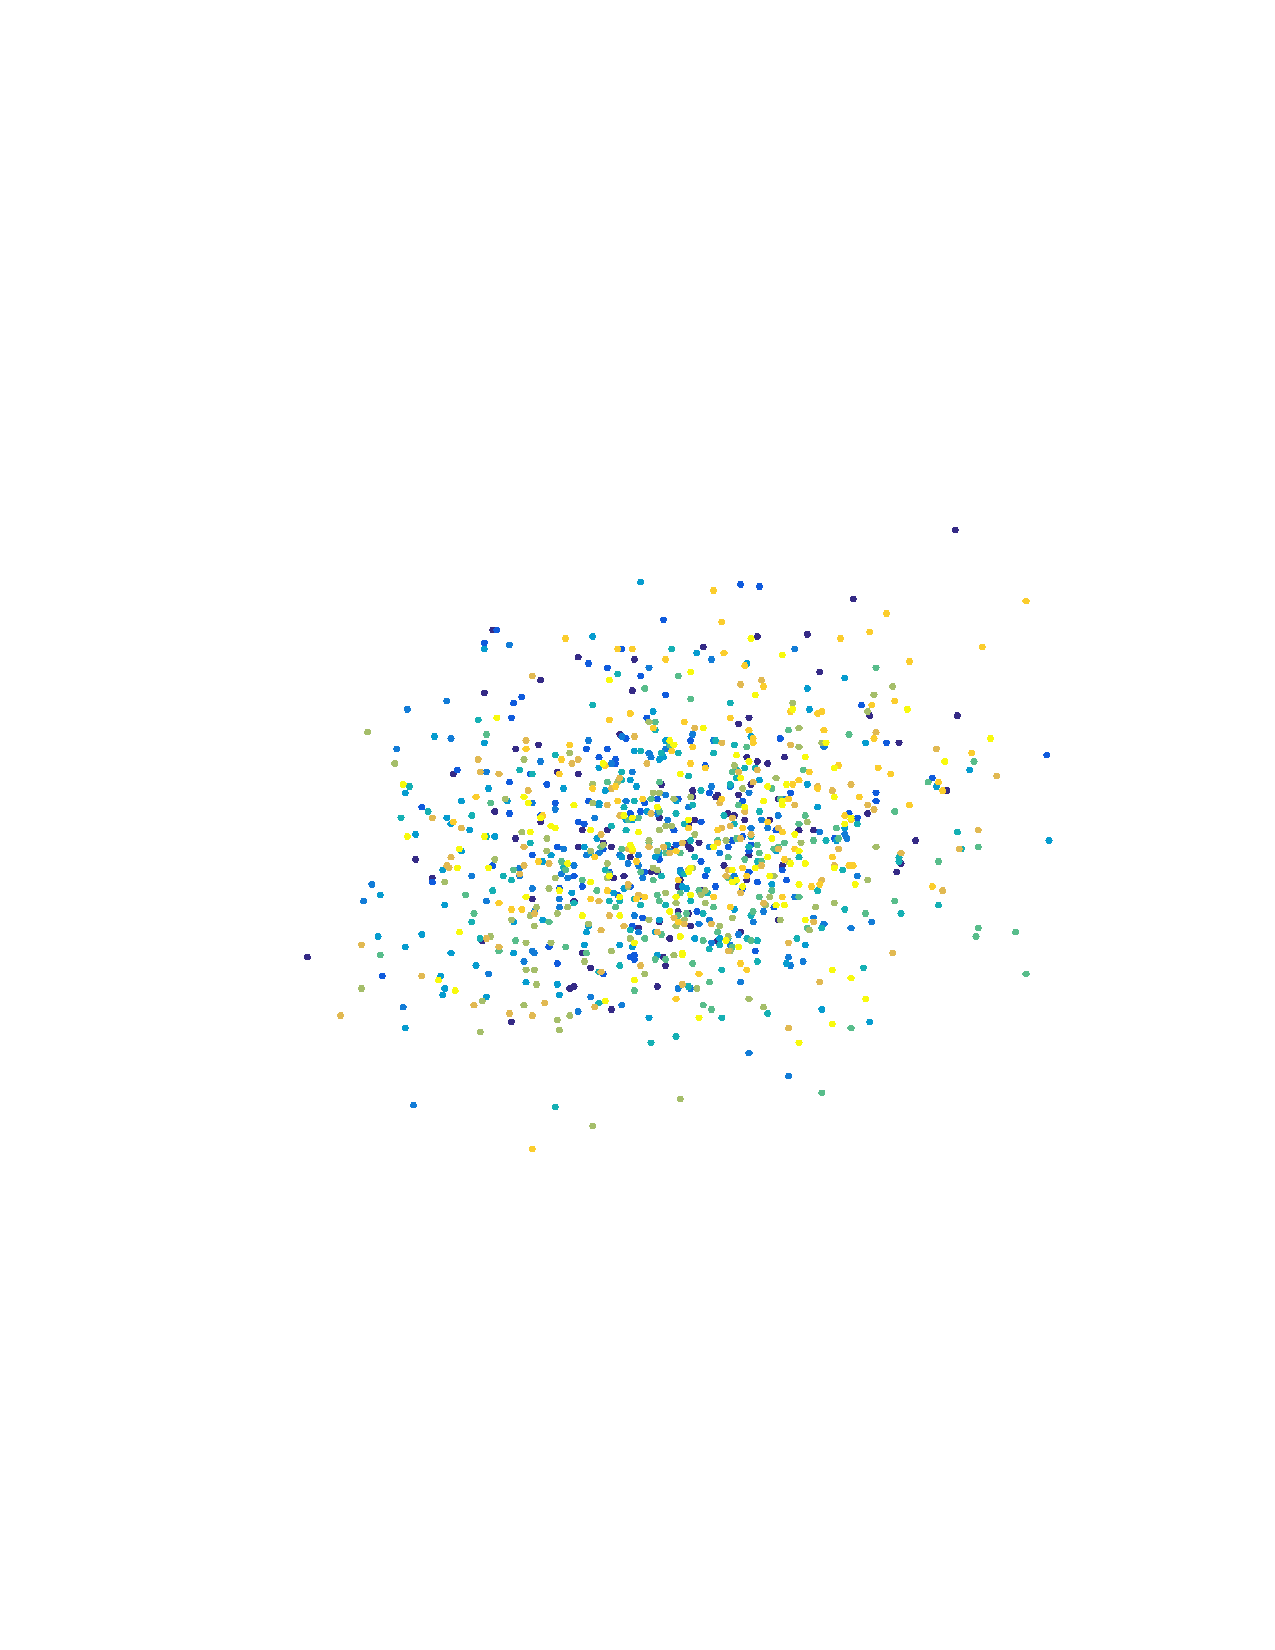
\includegraphics[width =0.27\textwidth]{jl.pdf}
 		}\qquad % space out the images a bit
 		\subfigure{%
 			\label{fig:pca}% label for this sub-figure
 			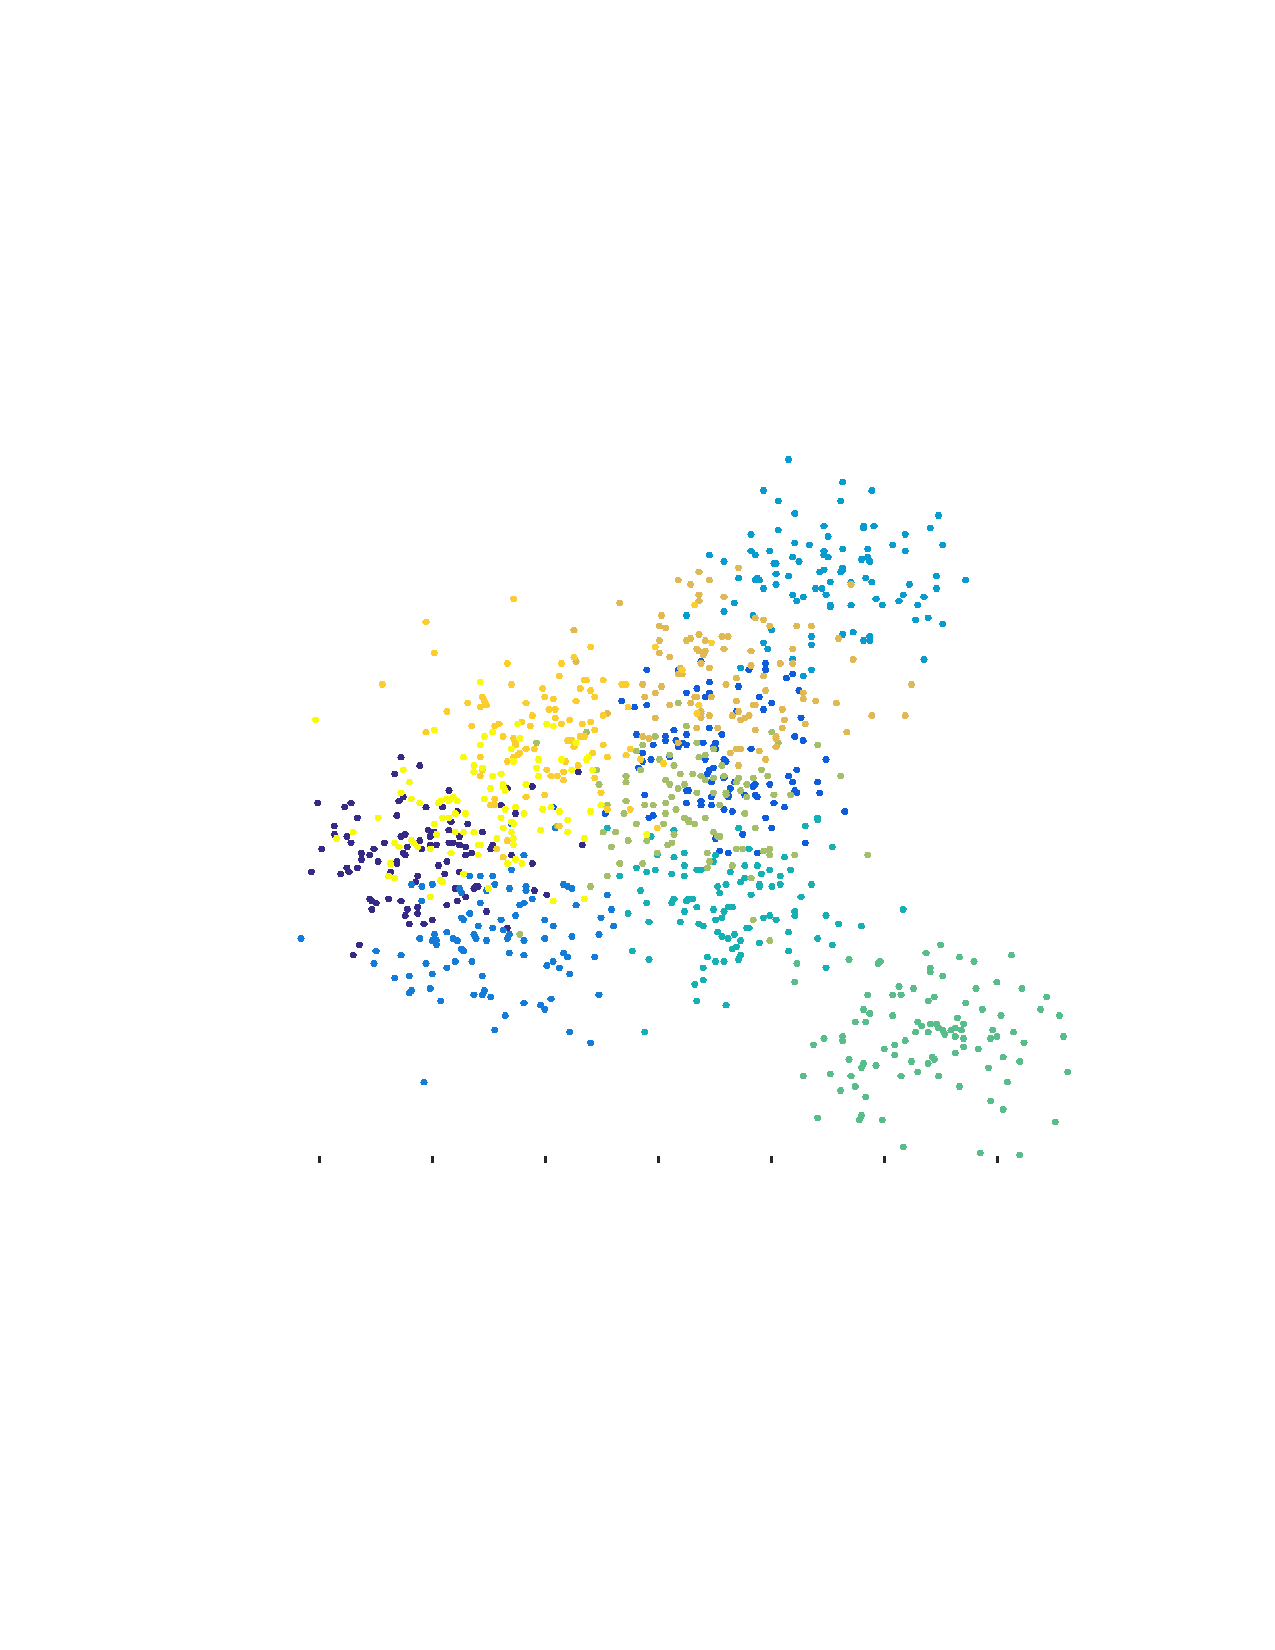
\includegraphics[width=0.27\textwidth]{pca.pdf}
 		}\qquad
 		\subfigure{%
 			\label{fig:tsne}% label for this sub-figure
 			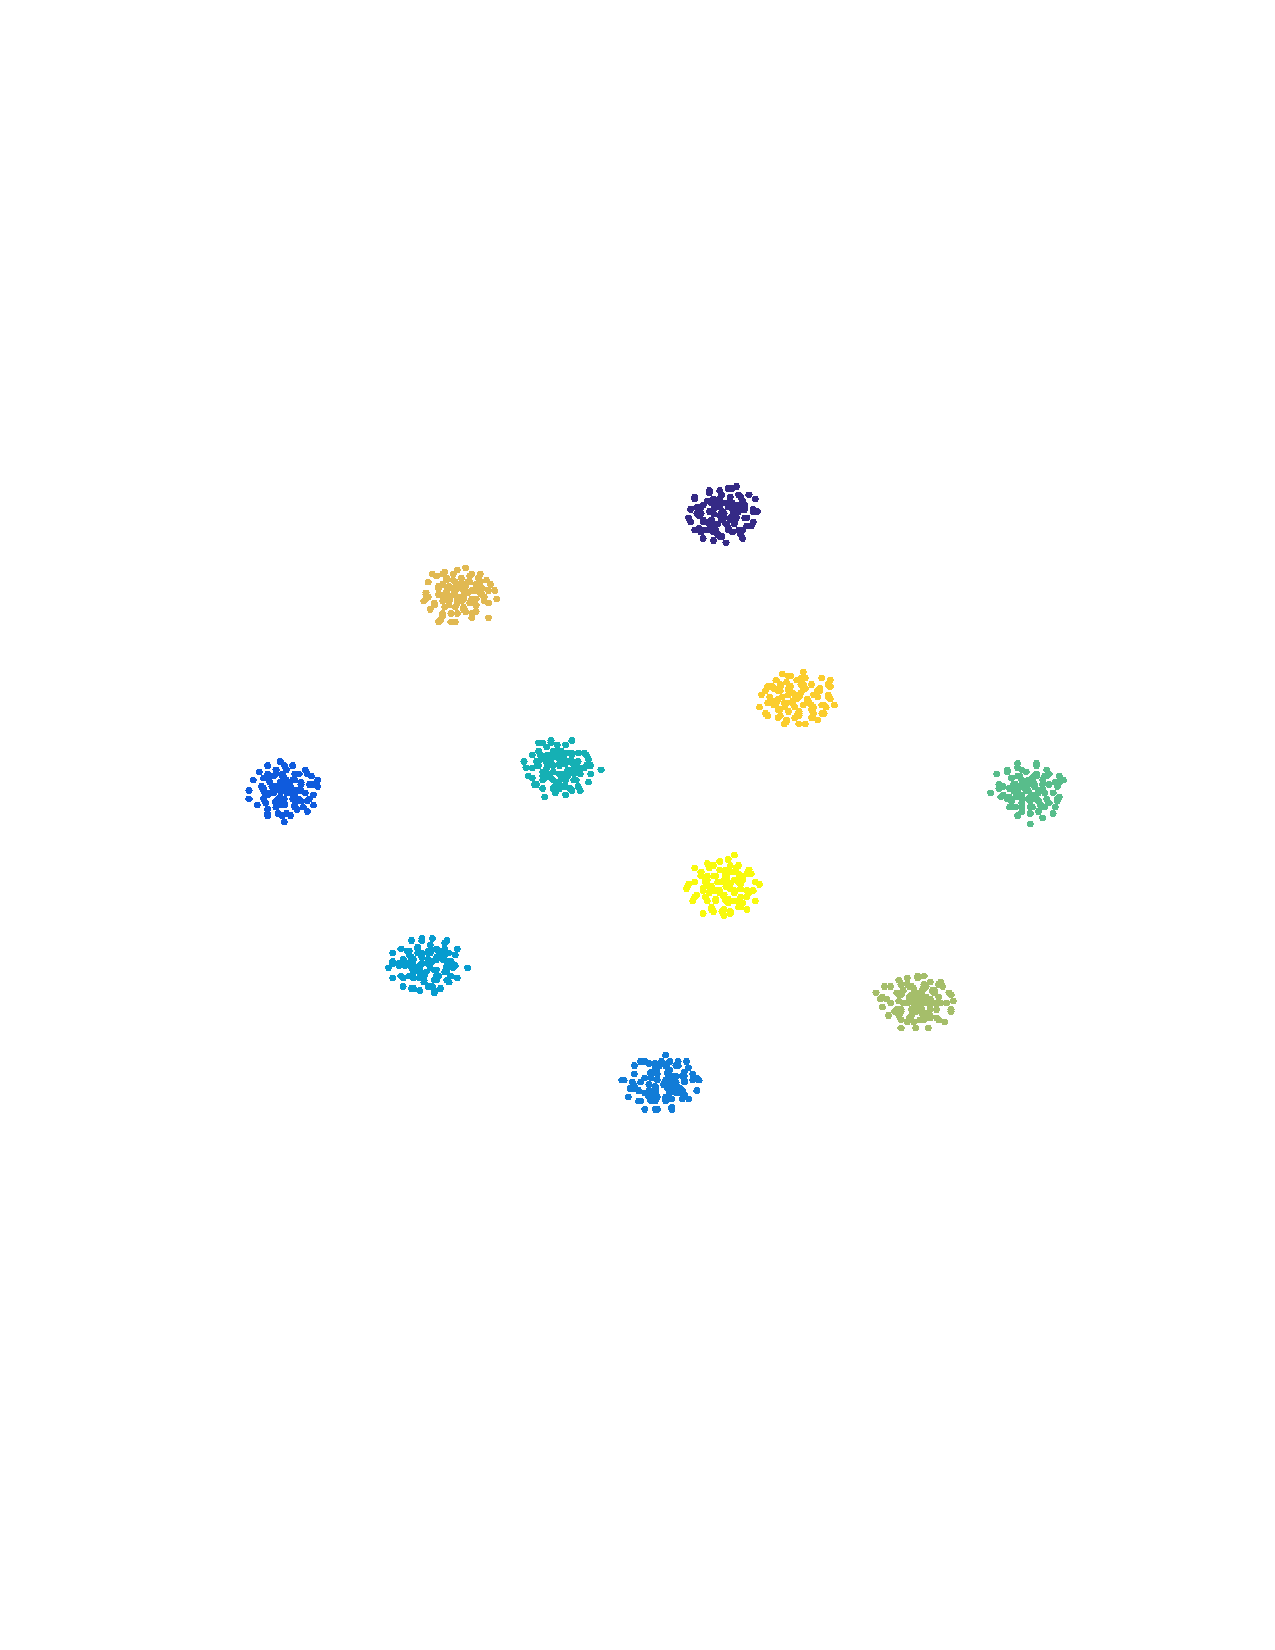
\includegraphics[width=0.27\textwidth]{tsne.pdf}
 		}\qquad
 		% \subfigure{%
 		%      \label{fig:uniqueness}% label for this sub-figure
 		%      \includegraphics[width=0.2\textwidth]{uniq_example.pdf}
 		% }
 	}
 \end{figure}
 
 
% \begin{figure}[htbp]
%%\floatconts
%	\label{fig:compare}% label for whole figure
%	{\caption{\small 2D embeddings of a mixture of 10 Gaussians with pairwise center separation $0.5\times$radius via: (a) random projection (JL), (b) projection to the subspace of top 2 singular vectors (PCA), (c) t-SNE.
%		}
%\centering
%  {%
%    \subfigure{
%    	%
%      \label{fig:JL}% label for this sub-figure
%      %\caption{text}
%      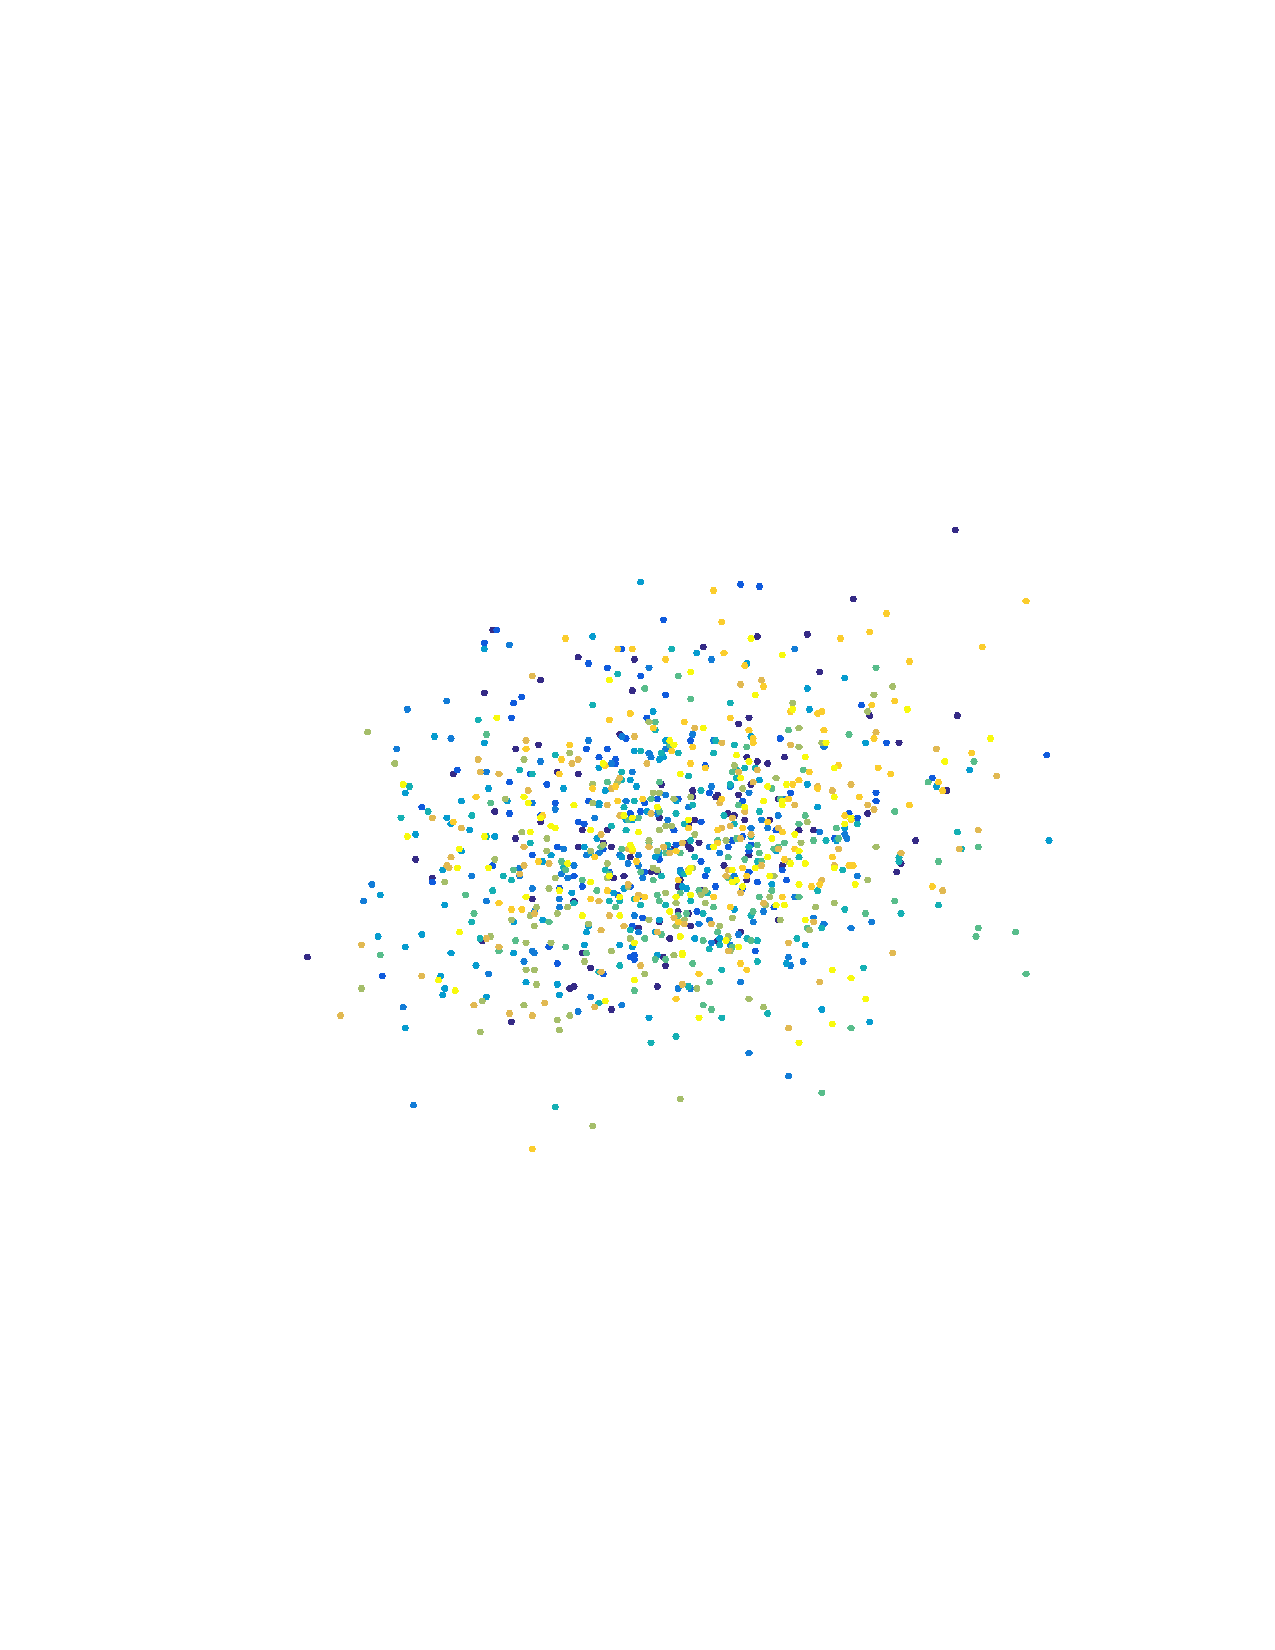
\includegraphics[width =0.27\textwidth]{jl.pdf}
%	}
%    \qquad % space out the images a bit
%    \subfigure{%
%      \label{fig:pca}% label for this sub-figure
%      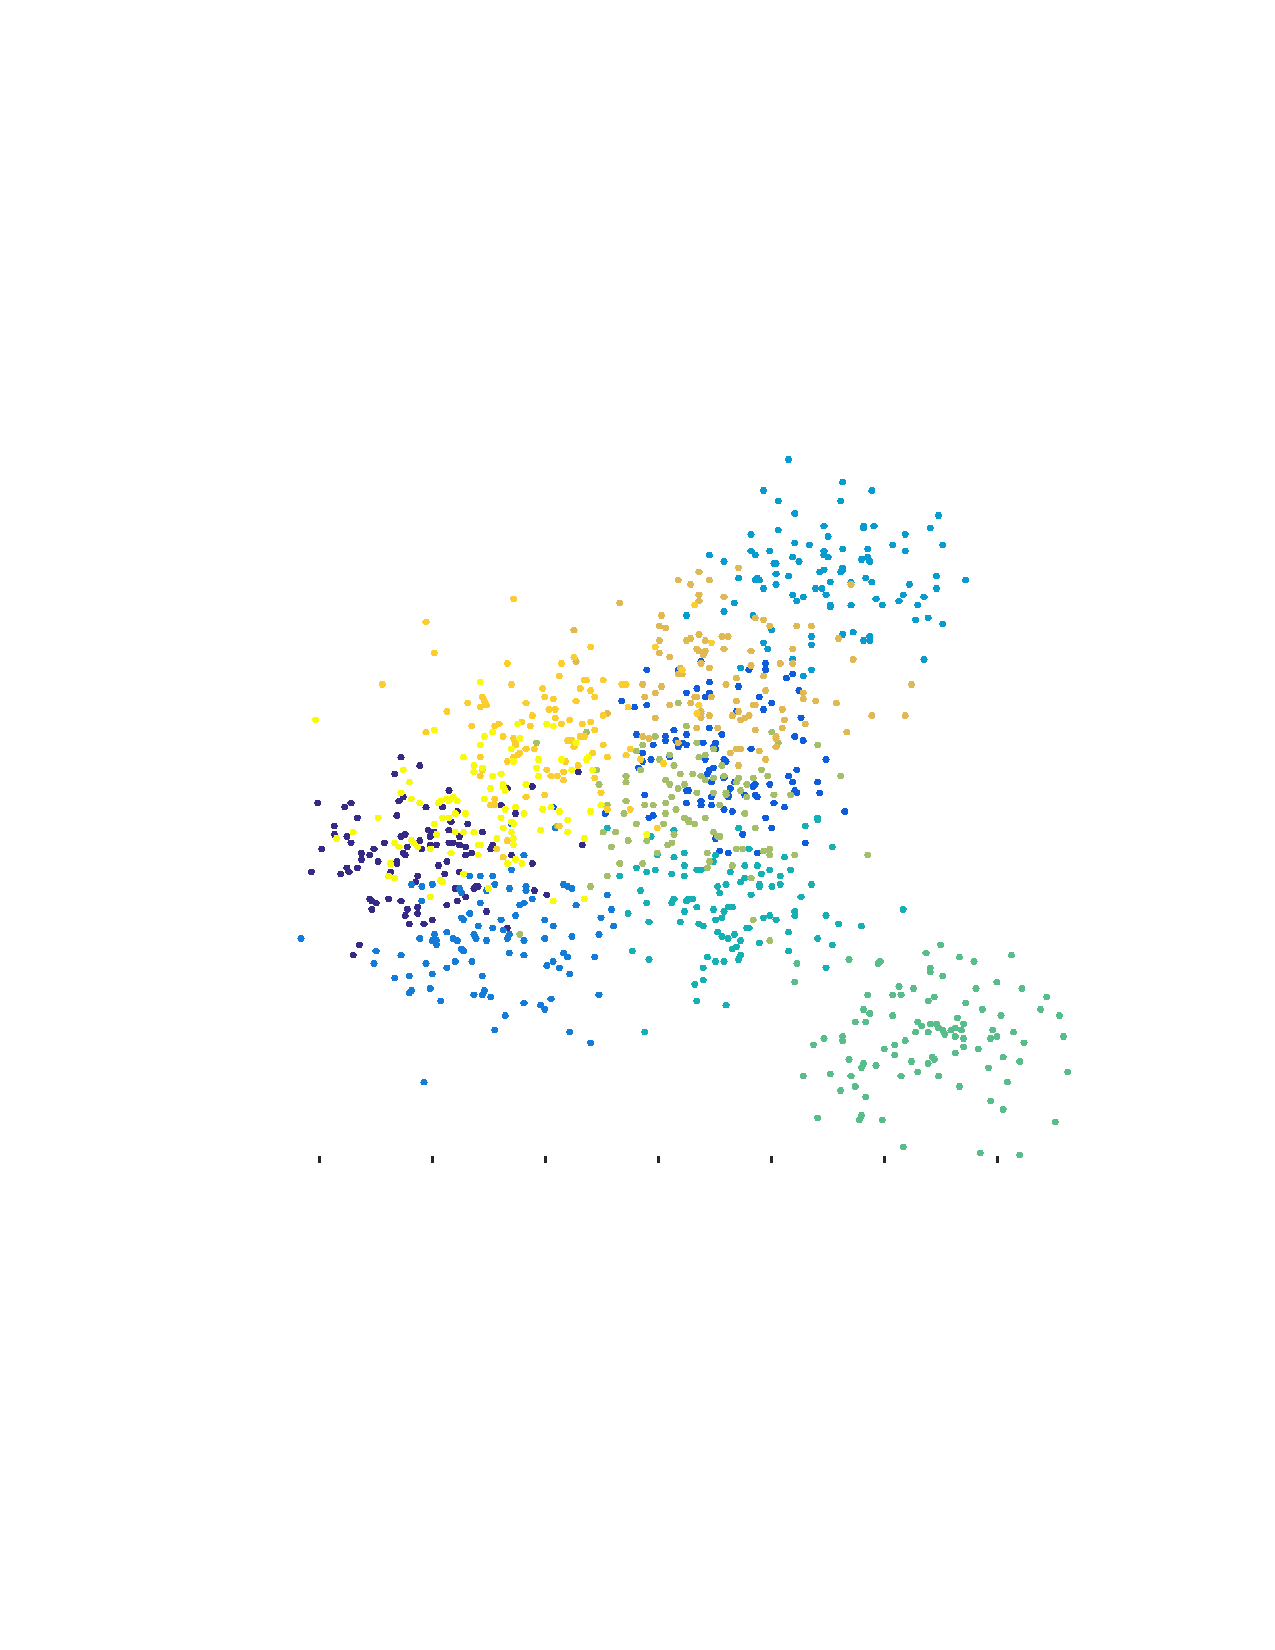
\includegraphics[width=0.27\textwidth]{pca.pdf}
%	}\qquad
%	 \subfigure{%
%      \label{fig:tsne}% label for this sub-figure
%      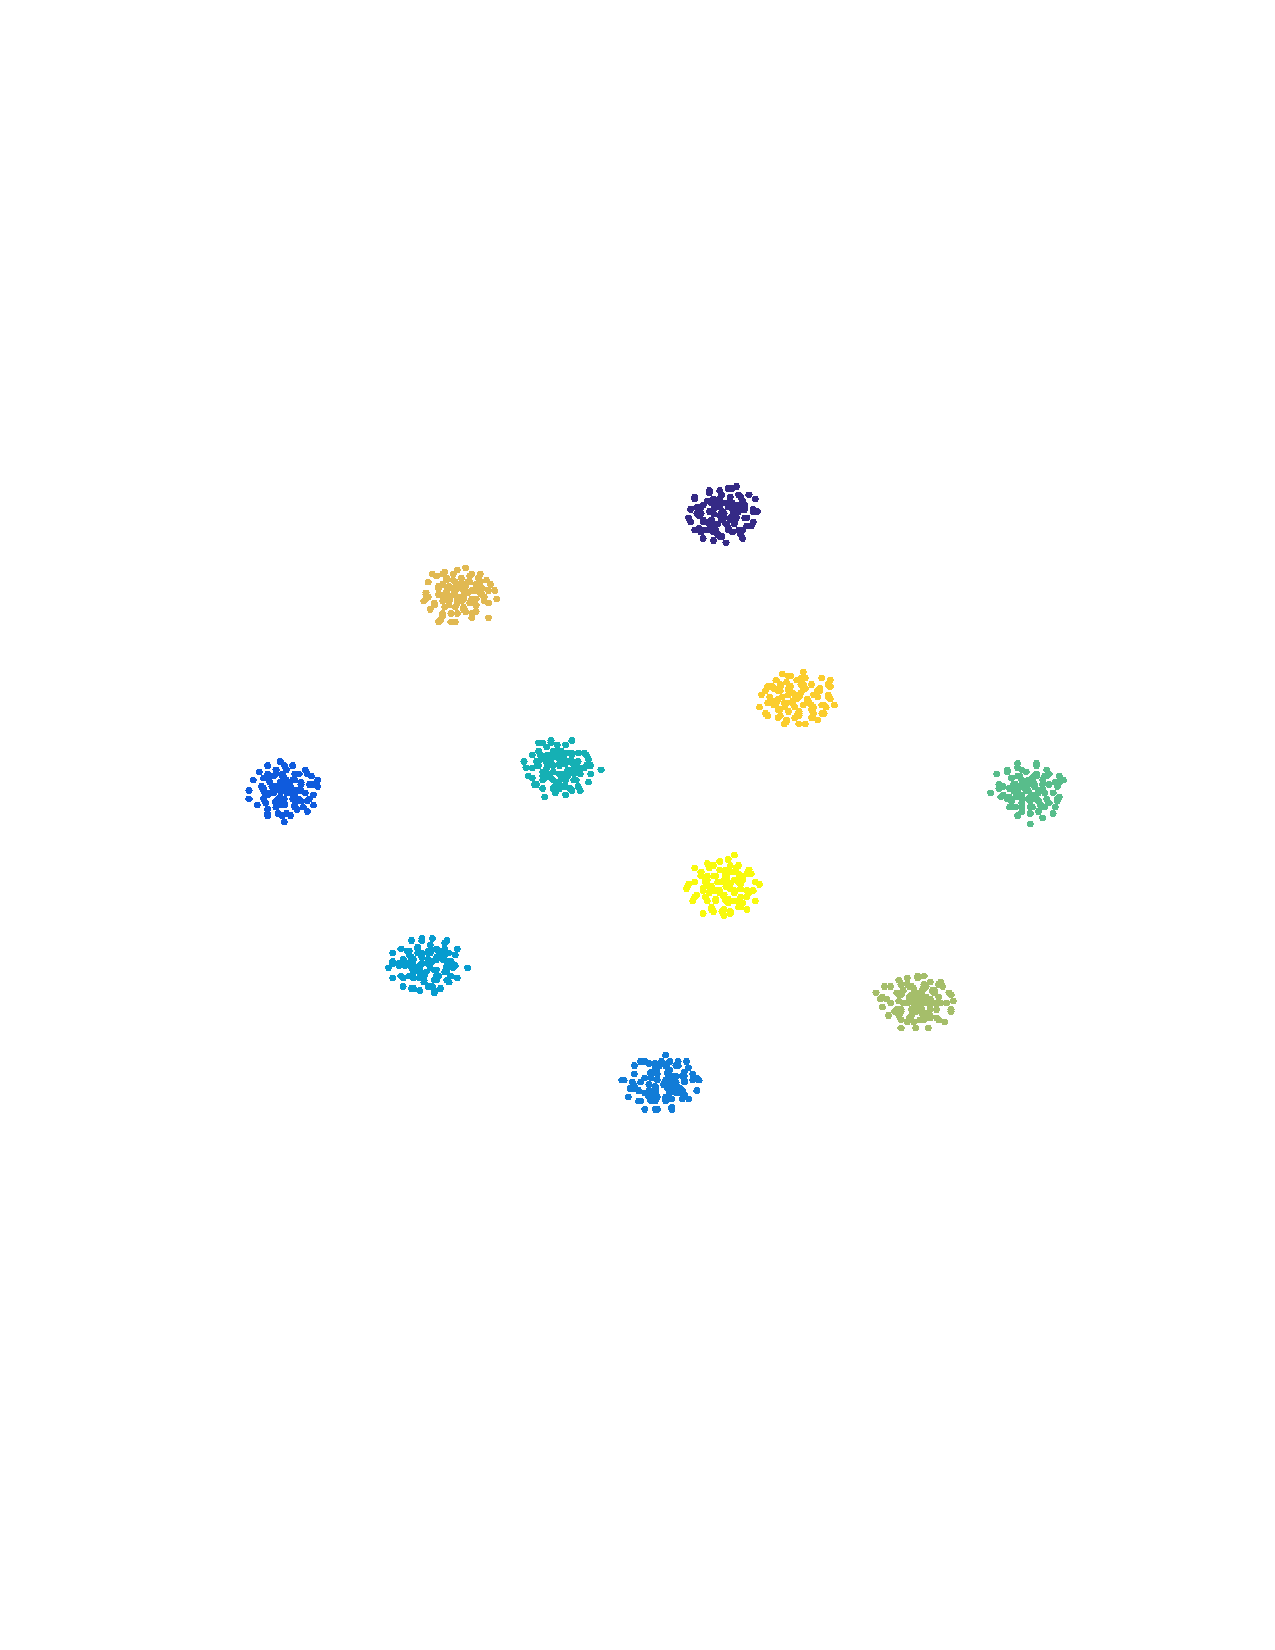
\includegraphics[width=0.27\textwidth]{tsne.pdf}
%	}\qquad
%	% \subfigure{%
% %      \label{fig:uniqueness}% label for this sub-figure
% %      \includegraphics[width=0.2\textwidth]{uniq_example.pdf}
%	% }
%	}
%}
%\end{figure}

%\begin{figure*}[t!]
%	\centering
%	\begin{subfigure}[t]{0.3\textwidth}
%		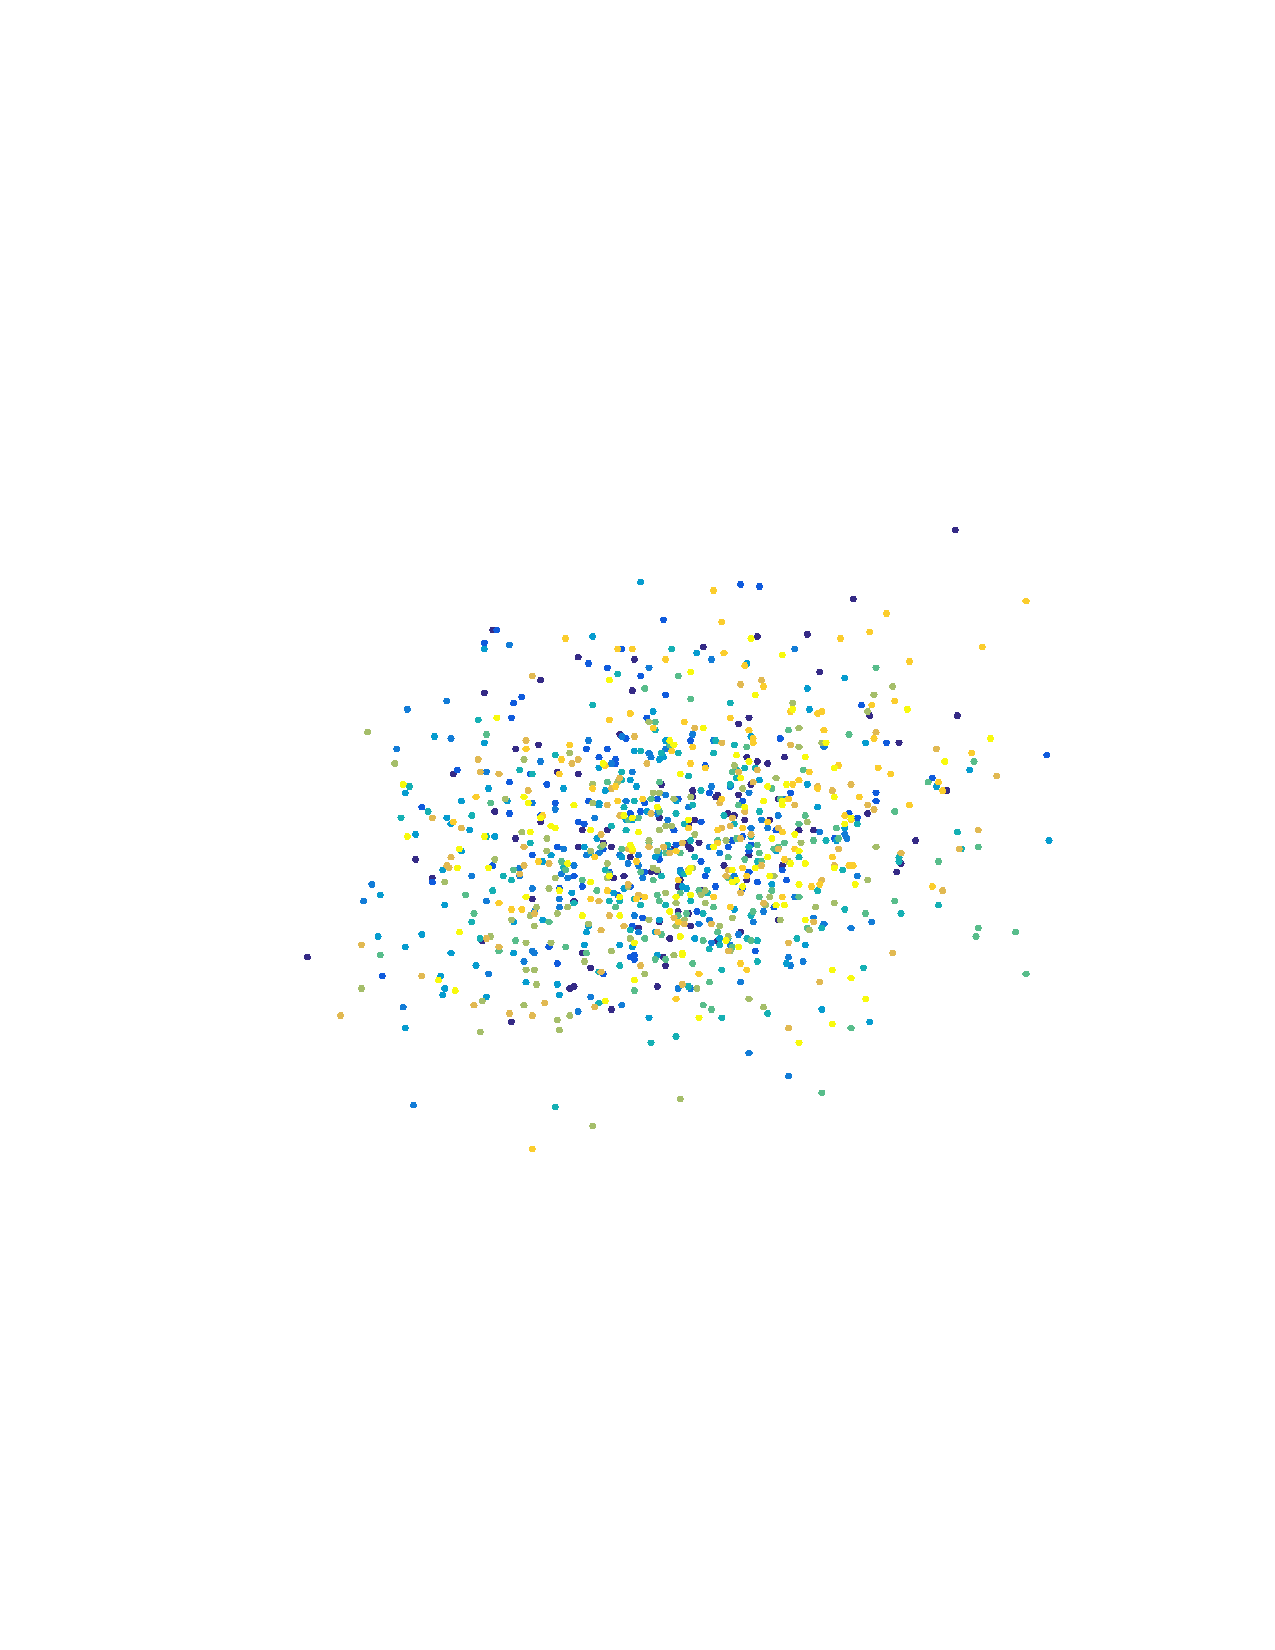
\includegraphics[width=\textwidth]{jl}
%		\caption{JL}
%	\end{subfigure}	
%	\quad
%	\begin{subfigure}[t]{0.3\textwidth}
%		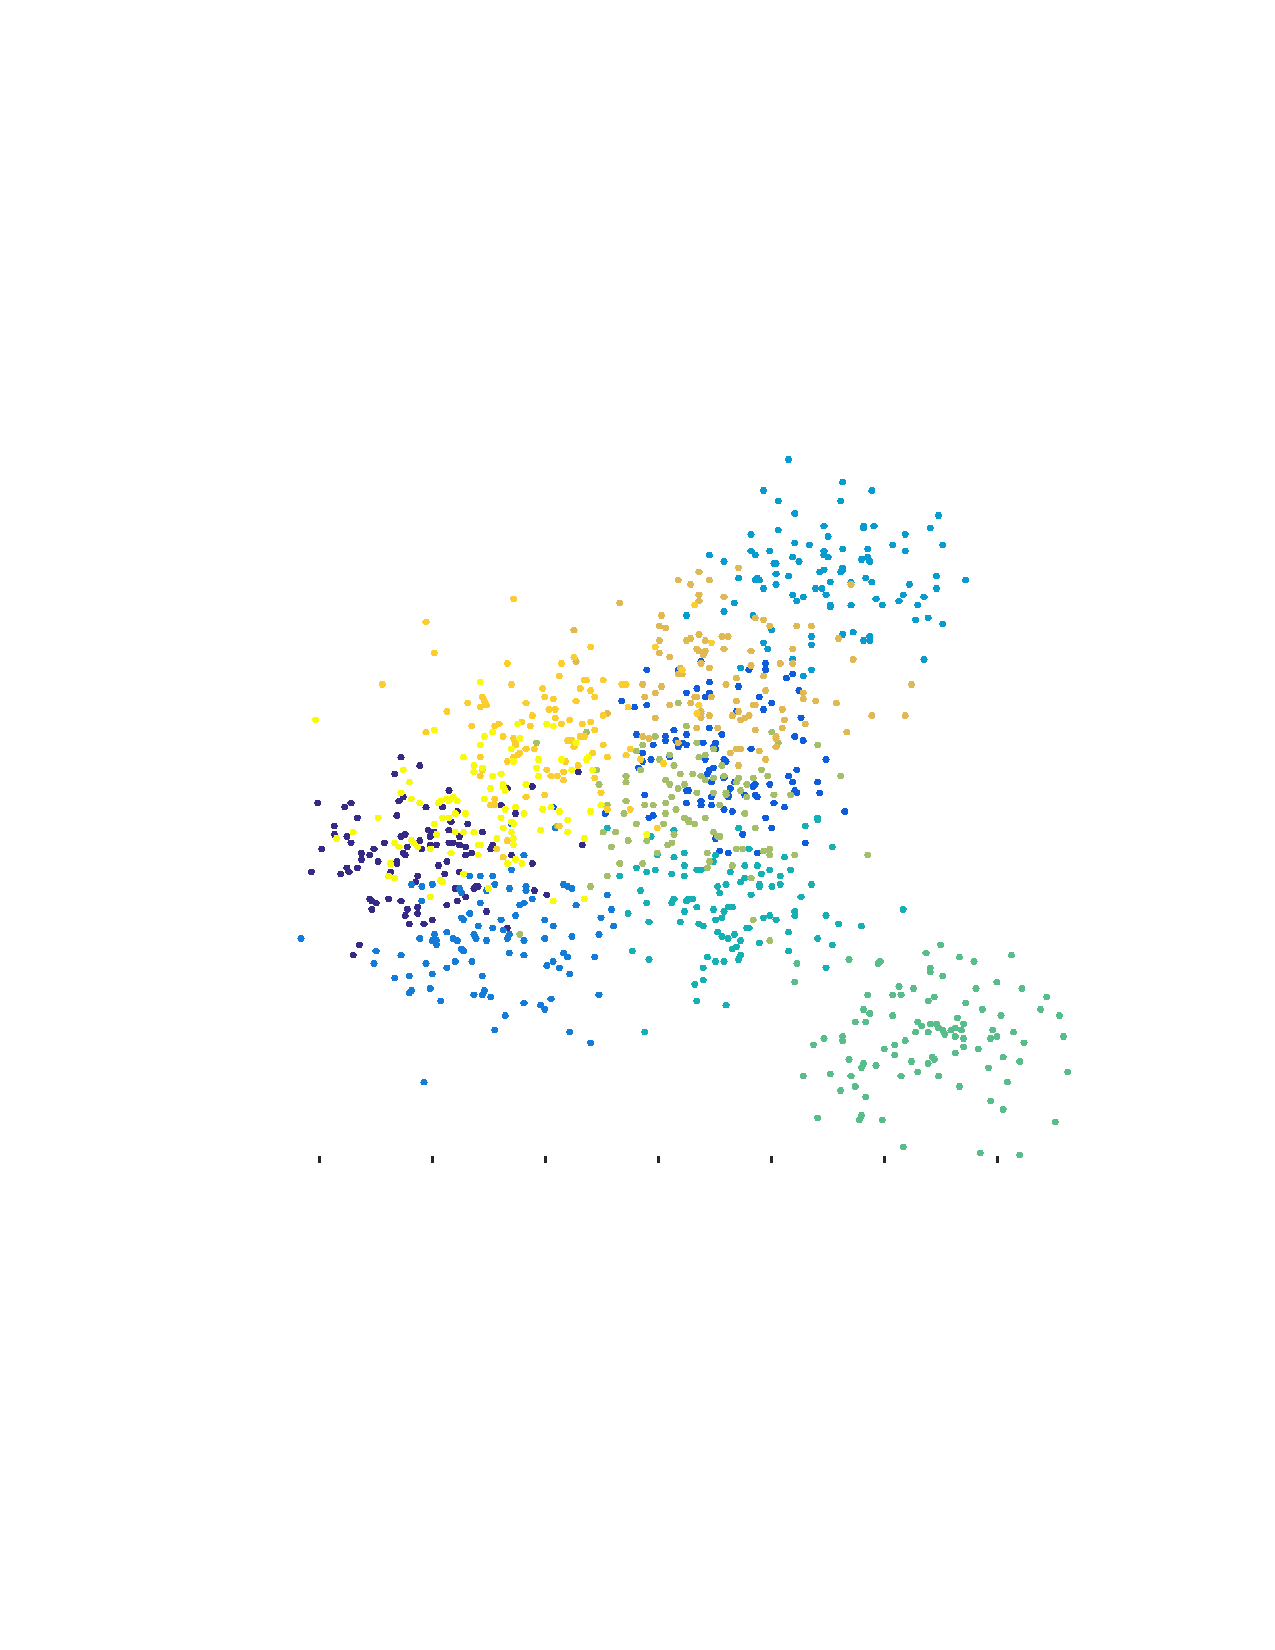
\includegraphics[width=\textwidth]{pca}
%		\caption{PCA}
%	\end{subfigure}
%	\quad
%	\begin{subfigure}[t]{0.3\textwidth}
%		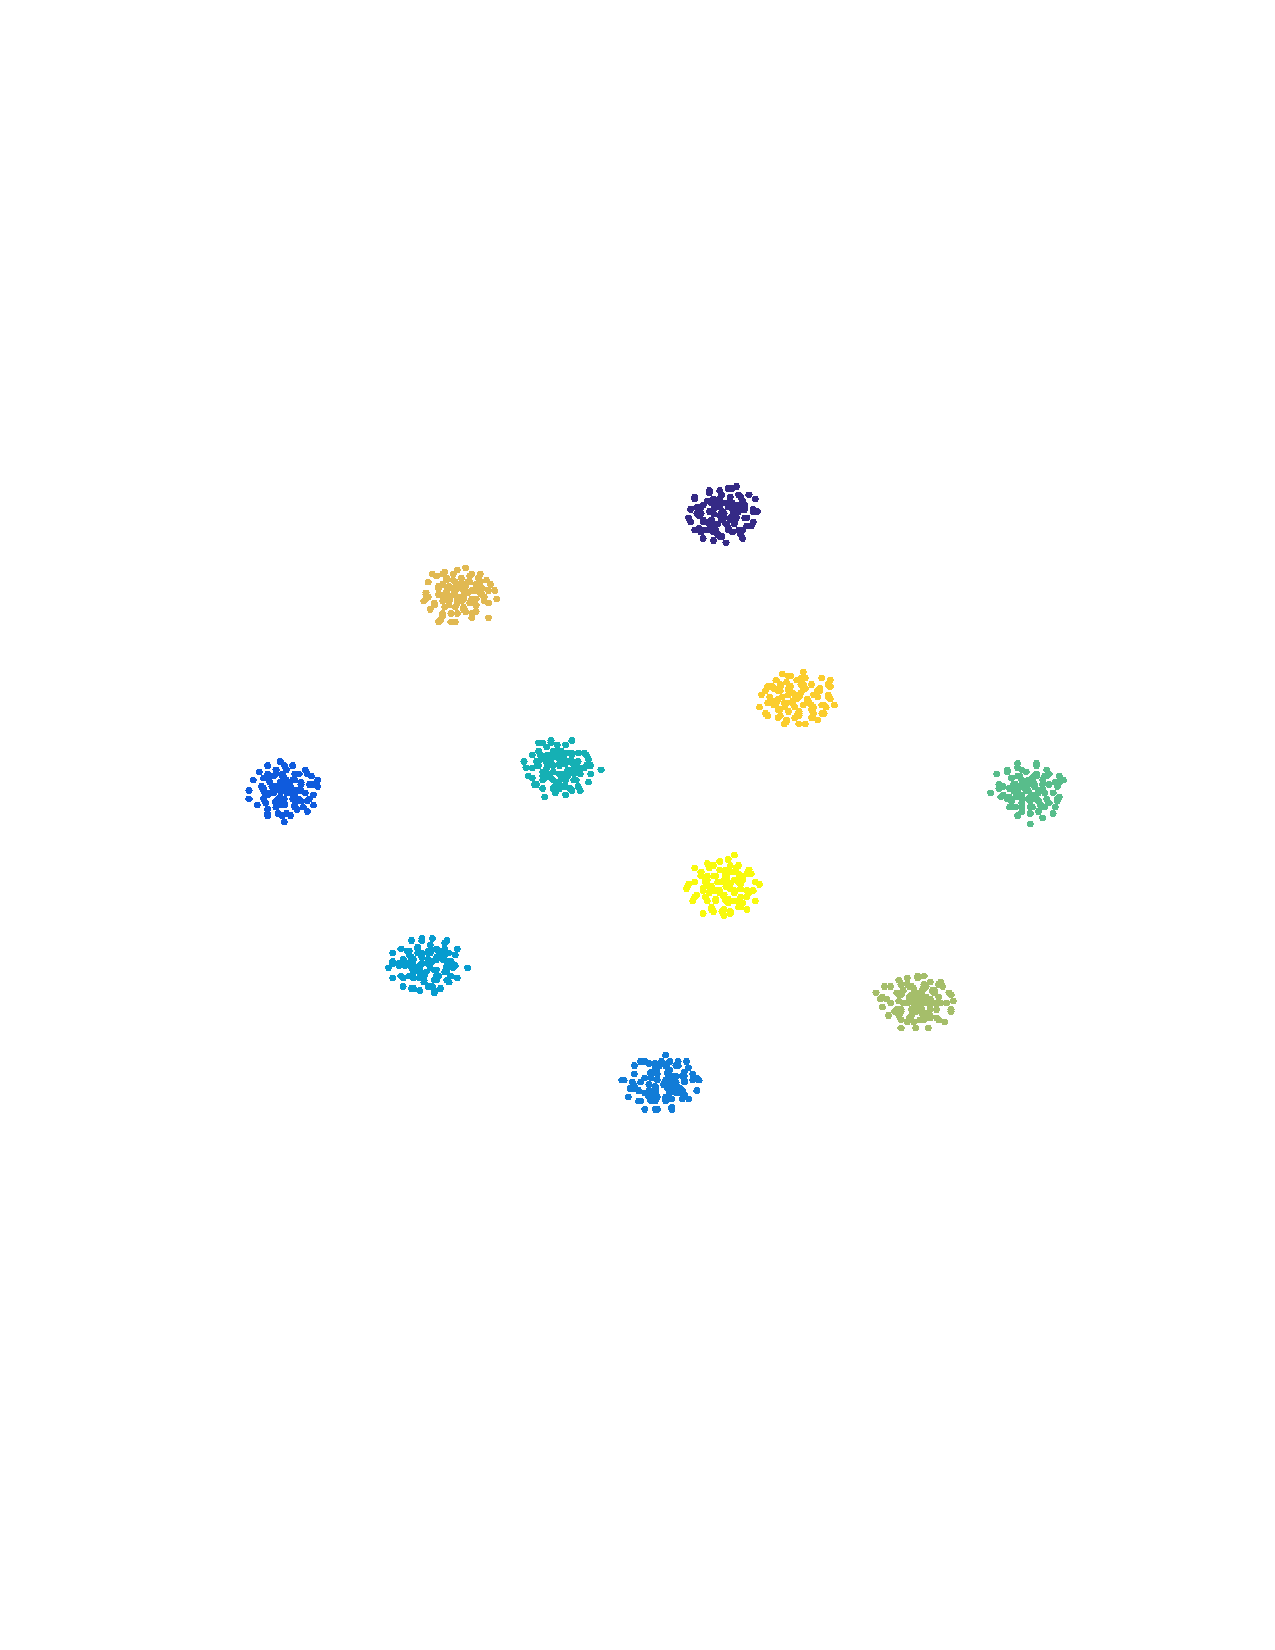
\includegraphics[width=\textwidth]{tsne}
%		\caption{t-SNE}
%			\label{fig:tsne}
%	\end{subfigure}
%	\vspace{10pt}
%	\caption{2D embeddings of a mixture of 10 Gaussians with pairwise center separation $0.5\times$radius via: (a) random projection (JL), (b) projection to the subspace of top 2 singular vectors (PCA), (c) t-SNE.
%	}
%	\label{fig:JLL}
%\end{figure*}


 %\begin{figure}[!tbp]
%   \centering
%   \subfloat[Flower one.]{\includegraphics[width=0.4\textwidth]{flower1.jpg}\label{fig:f1}}
%   \hfill
%   \subfloat[Flower two.]{\includegraphics[width=0.4\textwidth]{flower2.jpg}\label{fig:f2}}
%   \caption{My flowers.}
% \end{figure}

%   \includegraphics[width=.4\linewidth]{jl_2clusters.pdf}
%   \caption{Random 2D Projection of Mixture of 2 Gaussians}
%   \label{fig:sub1}
% \end{subfigure}%
% \begin{subfigure}{.5\textwidth}
%   \centering
%   \includegraphics[width=.4\linewidth]{jl_3clusters.pdf}
%   \caption{Random 2D Projection of Mixture of 3 Gaussians}
%   \label{fig:sub2}
% \end{subfigure}
% \label{fig:JL}
% \end{figure}
In 2008, \citet{van2008tsne} introduced a nonlinear algorithm, {\em t-Distributed Stochastic Neighbor Embedding or t-SNE} (an improvement over the earlier SNE algorithm of~\citet{DBLP:conf/nips/HintonR02}) for this task, which has become the de facto standard (see Figure~\ref{fig:tsne}) for visualizing high-dimensional datasets with diverse applications such as computer security~\citep{DBLP:conf/nca/GashiSLT09}, music analysis~\citep{conf/ismir/HamelE10}, cancer biology~\citep{Abdelmoula12244} and bioinformatics~\citep{WallachLilien2009}. % for the performance of t-SNE against the linear di

At a high level, t-SNE (like SNE) chooses two similarity measures between pairs of points - one for the high dimensional data and one for the 2-dimensional embedding. It then attempts to construct a 2-dimensional embedding that minimizes the KL divergence between
the vector of similarities between pairs of points in the original dataset
and the similarities between pairs of points in the embedding. This is a non-convex optimization problem and t-SNE employs gradient descent with random initialization (along with other tricks such as \emph{early exaggeration}) to compute a reasonable solution to it. See the full version of this paper for details. 

Of course, non-convex optimization drives much of today's progress in machine learning and data science, and thus poses a rich set of theoretical questions. Researchers have managed to rigorously analyze non-convex optimization algorithms in a host of settings~\citep{DBLP:conf/focs/Dasgupta99,MR3185945-Arora12,DBLP:conf/colt/AroraGM14,DBLP:conf/nips/BhojanapalliNS16,DBLP:conf/colt/GeHJY15,DBLP:journals/tit/SunQW17,DBLP:conf/icml/0001JZ17,DBLP:journals/corr/GeLM16,DBLP:conf/aistats/ParkKCS17}. These analyses usually involve making clean assumptions about the structure of data, usually with a generative model. The goal of the current paper is to rigorously analyze t-SNE in a similar vein. 

At the outset such a project runs into definitional issues about what a good {\em visualization} of clustering is. Many such issues are inherited from well-known issues in formalizing the goals of clustering~\citep{conf/nips/Kleinberg02}. In theoretical studies of clustering, such issues were sidestepped by going with a standard clustering formalization and assuming that data come with an (unknown) ground-truth clustering (for instance, mixtures of Gaussians, $k$-means, etc.). We make similar assumptions and assume that our goal is to produce a 2-dimensional embedding such that the points in the same clusters are noticeably closer together compared with points in different clusters. Under some of these standard models we show that t-SNE provably succeeds in computing a good visualization.  

% Since visualization appears closely related to dimensionality reduction, it is instructive to understand why standard dimensionality reduction techniques give poor solutions for the problem of data visualization. To gain intuition, let's also fix a simple model for clusterable data: a mixture of two isotropic gaussians with means separated by $\Delta$. Perhaps the simplest idea is to choose a random 2 dimensional projection to compute the visual embedding of the input data. In this case, it is not hard to see that such an embedding is a good visualization only in the special case when the two gaussian components are completely non overlapping (i.e., $\Delta \gg d^{1/2}$). On the other hand, having more than 2 clusters immediately precludes more adaptive embeddings such as by projecting to the subspace spanned by the top few singular vectors of the data matrix. In fact, in ,general, it's not hard to show that any 2 dimensional embedding that approximately preserves distances (up to scaling) for most pairs in the input data will fail for simple clusterable models such as well-separated mixtures of isotropic gaussians. In contrast, as we will show in this work, t-SNE constructs a non-linear embedding of the data that can produce faithful visualization of mixture of gaussians as long as the means are separated by $\Delta \gg d^{1/4}$. 


We emphasize that the focus of this paper is on formalizing the notion of visualization and providing a theoretical analysis of t-SNE. We do not advocate for t-SNE over other visualization methods.

We now begin by describing our formalization of the visualization problem followed by describing our results that give the first provable guarantees on t-SNE for computing visualization of clusterable data. 





%  The goal is to obtain an embedding such that nearby points in the dataset are mapped to nearby pints in the embedding while far-away points in the dataset are mapped to far-away points in the embedding. At a high level, t-SNE computes a similarity measure between every pair of points in the input data and attempts to construct a 2 dimensional representations such that the similarity measure of points in the 2 dimensional embedding roughly reflects the similarity measure of the corresponding points in the dataset.

% Given high-dimensional data $x_1, x_2, \ldots, x_n \in \R^d$, t-SNE computes a similarity measure $p_{i,j}$ for every pair of points. 




% The goal of this paper is to present a rigorous analysis of the t-SNE for the visualization problem. We formally identify

%  Perhaps unsurprisingly, even formalizing the problem of visualization runs into foundational issues and impossibility results such as those encountered in formalizing clustering. In order to circumvent such issues, we assume that there's a ground-truth cluster structure in the high-dimensional input data and focus on identifying 





% Data clustering is a basic primitive in both theoretical and practical unsupervised machine learning that focuses on grouping together data points into  subsets that are similar to each other. In many applications, we are interested in clustering the data in order to aid \emph{visualization} - finding a representation of the data in two or three dimensions that makes the underlying cluster structure \emph{visually} identifiable. Such methods form a first line of attack in exploratory data analysis and visualization in a range of fields including economics, biology, psychology and beyond\cite{??}. 

% While there are a myriad clustering methods \cite{??}, focusing on various theoretical and practical issues, most approaches do not naturally yield a low-dimensional representation of data that facilitates visualizing the cluster structure in the data. For example, a class of clustering methods identify a low-dimensional subspace that contains all the centers of individual clusters and then projects the data into such subspace. While this idea comes close, the number of clusters could easily exceed 2 or 3, the maximum limit of dimensions one can faithfully visualize, say on a computer screen. Indeed, this difficulty of visualizing cluster structure in low-dimensional appears, at least to some extent, inherent to such techniques. This is because these methods preserve, approximately and up to scaling, the distances between every pair of means. This, however, is provably impossible to ensure in a 2 or 3-dimensional embedding of the data. Thus visualizing cluster structure inherently appears to demand non-linear embeddings of high dimensional data. 

% While such issues have been scarcely examined in theoretical studies, there is an extremely popular non-linear heuristic developed by \cite{van2008tsne} called \emph{t-SNE} which produces a non-linear, 2 or 3-dimensional embedding of data that separates individual clusters in order to make them visually identifiable. For more than a decade, this technique has dominated...



\paragraph{Formalizing Visualization.}
\iffalse 
The input for t-SNE is a dataset that is ``clusterable.'' What does it mean for a dataset to be clusterable?
At a high-level, one imagines that there's some (application-dependent) similarity metric that one can then define clusterable data as a dataset that can be partitioned into groups such that points within a group are similar w.r.t. the metric while points in different groups are dissimilar. 


This paper assumes points come  that there is an unknown ``ground-truth'' clustering that implicitly induces a similarity metric.\fi
We assume that we are given a  collection of points $\cX = \{x_1, x_2, \ldots, x_n \} \subset \R^d$ and that there exists a ``ground-truth'' clustering described by a partition $\cC_1, \cC_2, \ldots, \cC_k$ of $[n]$ into $k$ clusters. 

%Next, we formalize the notion of \emph{visualization}.
A visualization is described by a 2-dimensional embedding $\cY = \{y_1, y_2, \ldots, y_n\} \subseteq \R^2$ of $\cX$, where each $x_i \in \cX$ is mapped to the corresponding $y_i \in \cY$. Intuitively, a cluster $\cC_\ell$ in the original data is \emph{visualized} if the corresponding points in the 2-dimensional embedding $\cY$ are well-separated from all the rest. The following definition formalizes this idea.


%In order for $\cY$ to be a \emph{visualization} of the given dataset $\cX$, we requi

\begin{defn}[Visible cluster]
Let $\cY$ be a 2-dimensional embedding of a dataset $\cX$ with ground-truth clustering $\cC_1, \ldots, \cC_k$.
Given $\epsilon \ge 0$, a cluster $\cC_\ell$ in $\cX$ is said to be $(1-\epsilon)$\emph{-visible} in $\cY$ if there exist $\cP, \cP_{\err} \subseteq [n]$ %with size $|\cP| = (1\pm 0.1)n/k$ 
such that:
\begin{enumerate}
\item $|(\cP\setminus \cC_{\ell}) \cup (\cC_{\ell}\setminus \cP)| \le \epsilon \cdot |\cC_{\ell}|$, $|\cP_\err|\le \epsilon n$, and % $|\cP \cap \cC_\ell| \geq (1-\epsilon) |\cC_\ell|$, and \wei{can change to $|(\cP\setminus \cC_{\ell}) \cup (\cC_{\ell}\setminus \cP)| \le \epsilon n$, then no need to have size constraint on $\cP$}
\item for every $i, {i'} \in \cP$ and $j  \in [n] \setminus (\cP\cup \cP_{\err})$, $\|y_i - y_{i'}\| \leq \frac12 \|y_i - y_j\|$. 
\end{enumerate}
In such a case, we say that $\cP$ $(1-\epsilon)$-\emph{visualizes} $\cC_i$ in $\cY$. %We will usually think of $\epsilon$ to be a fixed small constant say $0.01$ and write $\emph{visible}$ to mean $0.01$-approximately $\emph{visible}$.
%\wei{in our theorem $\epsilon = d^{-\nu}$}
	% For $\cP \subset \cS \subseteq [n]$, 
	% we say that $\cP$ is a \emph{visible cluster} in $\cS$ if for any $i, i' \in \cP$ and $j \in \cS \setminus \cP$, we have $\|y_i - y_{i'}\| \le \frac12 \|y_i - y_j\|$.
%	\begin{enumerate}[(i)]
%		\item $|\cP_{\err}| \le 0.01 |\cP|$;
%		\item For any $i, i' \in \cP$ and $j \notin \cP \cup \cP_\err$, we have 
%	\end{enumerate}
\end{defn}

% We are given a high-dimensional dataset $\cX = \left\{ x_1, x_2, \ldots, x_n \right\} \subset \R^d$.
% There is an unknown ground-truth clustering of the data points, denoted by a partition $\cC_1, \cC_2, \ldots, \cC_k$ of $[n]$, where $i \in \cC_\ell$ means that $x_i$ belongs to the $\ell$-th cluster.
%We assume that $k$ is a constant, 
% We assume that the dimension $d$ and the number of points $n$ are both sufficiently large, and $n=\poly(d)$.
% We also suppose that the numbers of points in all the clusters are close to each other; for simplicity, we assume 
% $ \frac{0.9n}{k} \le |\cC_{\ell}| \le \frac{1.1n}{k} $ for all $\ell\in[k]$.


% \Pnote{Add definitions for visualization, full and partial and justify.}

% definitions of visualization:

% Consider a two-dimensional embedding $\cY = \left\{ y_1, y_2, \ldots, y_n \right\} \subset \R^2$ of a dataset $\cX = \left\{ x_1, x_2, \ldots, x_n \right\} \subset \R^d$.

It is now easy to define when $\cY$ is a good \emph{visualization} - we ask that every cluster $\cC_\ell$ in the dataset $\cX$ is visualized in $\cY$.

\begin{defn}[Visualization] \label{def:visualization-full}
	Let $\cY$ be a 2-dimensional embedding of a dataset $\cX$ with ground-truth clustering $\cC_1, \ldots, \cC_k$. % for $1 \leq i \leq k$.
	Given $\epsilon\ge0$,
	we say that $\cY$ is a \emph{$(1-\epsilon)$-visualization} of $\cX$
	 if 
	there exists a partition $\cP_1, \cP_2, \ldots, \cP_k, \cP_{\err}$ of $ [n]$ such that:
	\begin{enumerate}[(i)]
		\item For each $i \in [k]$, $\cP_{i}$ $(1-\epsilon)$-visualizes $\cC_i$ in $\cY$, and
		%$\|y_i - y_{i'}\| \le \frac12 \|y_i - y_j\|$, $\forall i, i' \in \cP_{\ell}, j\in \cP_{\ell'}$, $\forall \ell, \ell' \in [k]$ ($\ell\not=\ell'$).
		%For any $\ell, \ell' \in [k]$ ($\ell\not=\ell'$) and any $i, i' \in \cP_{\ell}, j\in \cP_{\ell'}$, we have $\|y_i - y_{i'}\| \le \frac12 \|y_i - y_j\|$, and
		\item %$\frac{0.9n}{k} \le |\cP_{\ell}| \le \frac{1.1n}{k}$ for all $\ell \in [k]$, and
		 $|\cP_{\err}| \le \epsilon n$.
	\end{enumerate}
In particular, when $\epsilon = 0$, we say that $\cY$ is a \emph{full visualization} of $\cX$.
%In particular, when $\epsilon=0$, we say that $\cY$ is a full visualization of $\cX$.
	%\wei{We can prove a result with $\epsilon=0$. Maybe remove the error in the definition?}
\end{defn}


%\vspace{-5mm}
\begin{remark*}
 Note that this formalization of visualization should be considered a first cut, since ultimately human psychology must come into play. For instance, humans may reasonably visualize two parallel lines as two clusters, but these violate our definition.

 A natural question is whether clustering inferred from a visualization is unique. Our definition above does not guarantee this. Indeed, this is inherently impossible and relates to the ambiguity in the definition of clustering: for example, it can be impossible to determine whether a given set of points should be viewed as one cluster or two different smaller clusters. See Figure~\ref{fig:unique-clustering} for an example.
% For e.g., observe that there are two equally reasonable ways to interpret Figure  as a visualization of 3 high dimensional clusters.

It is, however, not hard to establish that under an additional assumption that the size (number of points) of any cluster is smaller than twice the size of any other, full visualization as defined in Definition \ref{def:visualization-full} uniquely determines a clustering.
\end{remark*}

\begin{figure}[htbp]
	%\floatconts
	\centering
	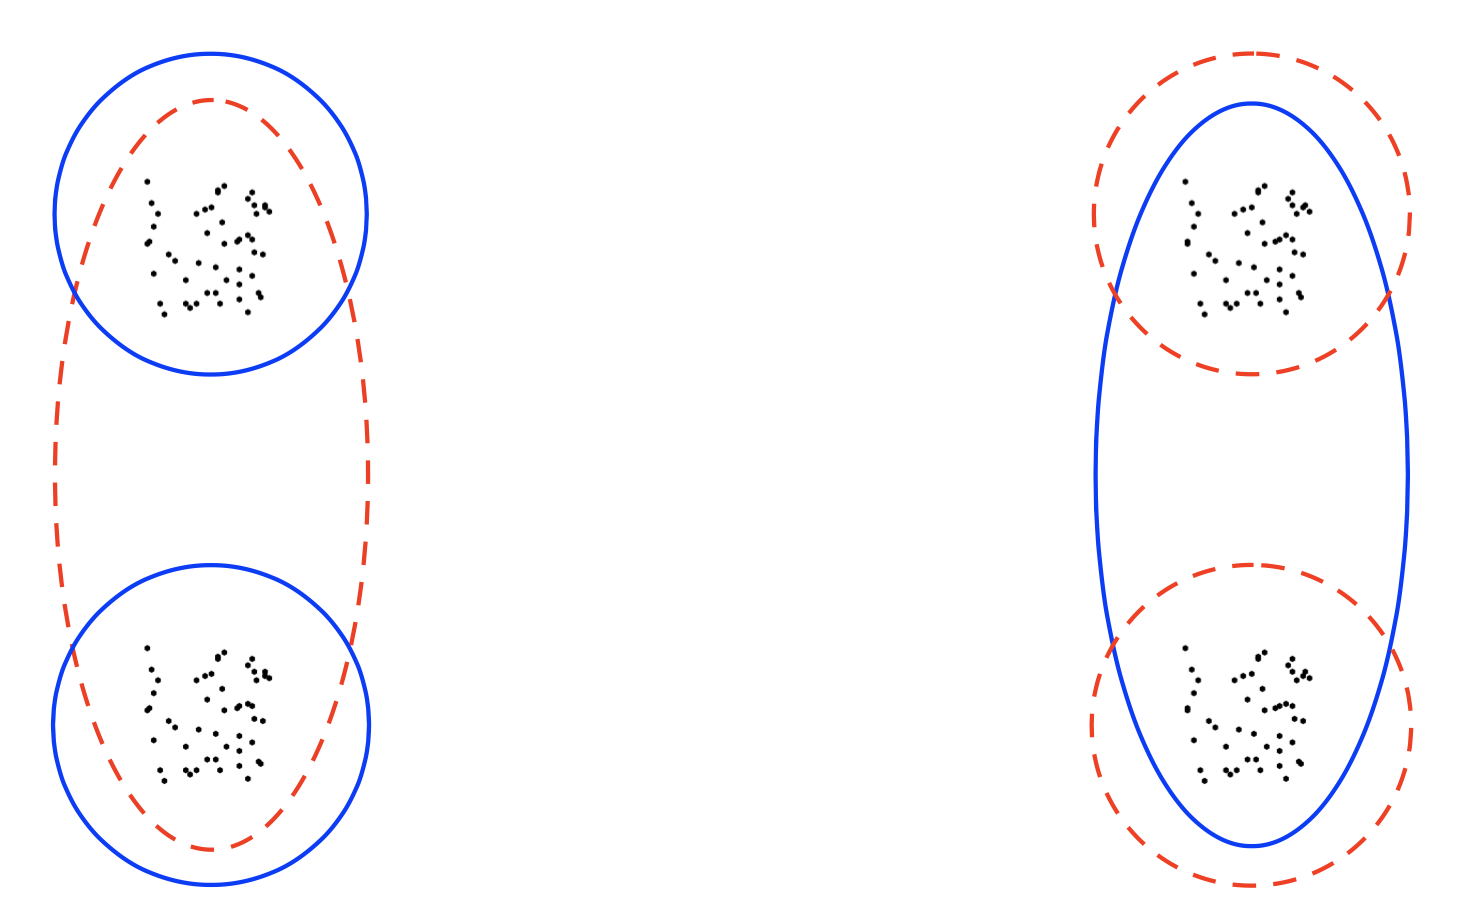
\includegraphics[width =0.35\textwidth]{unique_example.png}
	\vspace{10pt}
	\caption{If we knew that there are 3 clusters in the original data, the blue and red outlines denote equally valid guesses for the underlying clustering based on the above visualization.}% caption command
	\label{fig:unique-clustering}% label
\end{figure}


In order to study fine-grained behaviors of t-SNE, we also define a weaker variant of visualization where at least one cluster is visualized.% (but not all). 

\begin{defn}[Partial visualization] \label{def:visualization-partial}
	Given $\epsilon\ge0$, we say that $\cY$ is a \emph{$(1-\epsilon)$-partial visualization} of $\cX$ if 
	there exists a subset $\cP \subseteq [n]$ such that $\cP$ $(1-\epsilon)$-visualizes $\cC_\ell$ for some $\ell\in[k]$. 
	% \begin{enumerate}[(i)]
	% 	\item $\cP$ is a visible cluster in $[n] \setminus \cP_{\err}$;
	% 	%$\|y_i - y_{i'}\| \le \frac12 \|y_i - y_j\|$, $\forall i, i' \in \cP_{\ell}, j\in \cP_{\ell'}$, $\forall \ell, \ell' \in [k]$ ($\ell\not=\ell'$).
	% 	%For any $i, i' \in \cP, j\in [n] \setminus (\cP \cup \cP_{\err})$, we have $\|y_i - y_{i'}\| \le \frac12 \|y_i - y_j\|$.
	% 	\item $\frac{0.9n}{k} \le |\cP| \le \frac{1.1n}{k}$ and $|\cP_{\err}| \le \epsilon n$.
	% \end{enumerate}
\end{defn}



\subsection{Our Results}

Our main result identifies a simple deterministic condition on the clusterable data under which t-SNE provably succeeds in computing a full visualization. 

%\Pnote{I have removed the balancedness condition below. Full Visualization section needs an update.}

\begin{defn}[Well-separated, spherical data] \label{def:sperical-separated-intro}
	Let $\cX = \{ x_1, x_2, \ldots, x_n \} \subset \R^d$ be clusterable data with $\cC_1, \cC_2,\ldots, \cC_k$ defining the individual clusters such that for each $\ell\in[k]$, $|\cC_\ell| \ge 0.1 (n/k)$. 
	We say that $\cX$ is $\gamma$-spherical and $\gamma$-well-separated if for some $b_1, b_2, \ldots, b_k>0$, we have:
	\begin{enumerate}
		\item $\gamma$-\textbf{Spherical: } For any $ \ell \in [k]$ and $i, j \in \cC_{\ell}$ ($i\not=j$), we have $\| x_i - x_j \|^2 \ge \frac{b_\ell}{1+\gamma}$, and for any $i\in \cC_{\ell}$ we have $\left| \left\{ j \in \cC_{\ell} \setminus\{i\}: \norm{x_i-x_j}^2 \le b_\ell \right\} \right| \ge 0.51 |C_{\ell}|$.
		\item $\gamma$-\textbf{Well-separated: } For any $\ell, \ell' \in [k]$ ($\ell\not=\ell'$), $i \in \cC_{\ell}$ and $j\in \cC_{\ell'}$ we have $\| x_i - x_j \|^2 \ge  (1+ \gamma \log n)  \max\{b_\ell, b_{\ell'}\}$.
	\end{enumerate}
\end{defn}

The first condition asks for the distances between points in the same cluster (``intra-cluster distances'') to be concentrated around a single value (with $\gamma$ controlling the ``amount'' of concentration). The second condition requires that the distances between two points from different clusters should be somewhat larger than the intra-cluster distances for each of the two clusters involved. In addition, we require that none of the clusters has too few points. Such assumptions are satisfied by well-studied probabilistic generative models for clusterable data such as mixture of Gaussians and more generally, mixture of log-concave distributions, and have been used in previous work \citep{DBLP:conf/focs/Dasgupta99,arora2005learning} studying ``distance-based'' clustering algorithms.  


% Minor variants of such conditions appear in previous work on data clustering based on pairwise distances . This means that we would like the pairwise distances $\|x_i - x_j\|$ for all $i, j\in \cC_{\ell}$ ($i\not=j$) to be tightly concentrated. It is particularly interesting when $\gamma \log n \ll 1$ - in this case we only require the distance from $x_i$ to any point from a different cluster to be slightly larger than its distance to most points from the same cluster.
% This can be satisfied when the data come from a mixture of Gaussians, or more generally, a mixture of log-concave distributions.

% \begin{remark*}
% 	\wei{remark about the definition $\gamma$-spherical, compare with ``spherical Gaussian''}
% \end{remark*}
For spherical and well-separated data, our main theorem below shows that t-SNE with early exaggeration succeeds in finding a full visualization.   

\begin{thm}[Informal] \label{thm:full-vis-main-intro}
	%Let $\eta>0$ be a constant.
	Let $\cX = \{x_1, x_2, \ldots, x_n\} \subset \R^d$ be $\gamma$-spherical and $\gamma$-well-separated clusterable data with $\cC_1, \cC_2,\ldots, \cC_k$ defining the individual clusters. 
	%$a_1, \ldots, a_k, b_1, \ldots, b_k>0$ 
	%   such that:
	% \begin{enumerate}[(a)]
	% 	\item \label{item:gamma-spherical} ($\gamma$-spherical);
	% 	%\item \label{item:distance-ub} for any $\ell \in [k]$ and $i \in \cC_{\ell}$, we have $\left| \left\{ j\sim i, j\not=i: \norm{x_i-x_j}^2 \le b_\ell \right\} \right| \ge \left( \frac12 + \eta \right) |C_{\pi(i)}|$;
	% 	\item \label{item:separation} (separation) 
	% \end{enumerate}
	Then, t-SNE with early exaggeration on input $\cX$ outputs a full visualization of $\cX$ with high probability.  
	%Suppose in t-SNE
	%we set $\tau_i^2 = \frac\gamma4 \cdot \min_{j\in[n]\setminus\{i\}} \|x_i - x_j\|^2$ in \eqref{eqn:def-p} for each $i\in[n]$, and choose $\sqrt{k^3n}\log n \ll \alpha \le \rho n$ (for some sufficiently small constant $\rho$) and $h = 1$.
	%Then if we initialize t-SNE by generating $\left\{y_i^{(0)}: i\in[n]\right\}$ i.i.d. from the uniform distribution over $[-0.01, 0.01]^2$, after running t-SNE for $T = \Theta\left( \frac{n\log n}{\alpha} \right)$ iterations, $\cY^{(T)} = \left\{y_1^{(T)}, \ldots, y_n^{(T)}\right\}$ will with high probability be a full visualization of $\cX$ with visible clusters $\cC_1, \ldots, \cC_k$.
	%all the four conditions in Theorem~\ref{thm:full-vis-pij-condition} can be satisfied.
	%	\begin{equation*}
	%	\begin{aligned}
	%	a_\ell \le \| x_i - x_j \|^2 \le b_\ell, & \qquad \forall \ell \in [k], \forall i, j \in \cC_{\ell} \ (i\not=j), \\
	%	\| x_i - x_j \|^2 \ge  (2\gamma \log n + 1)  b_\ell, & \qquad \forall \ell \in [k], \forall i \in \cC_{\ell}, \forall j\notin \cC_{\ell}.
	%	\end{aligned}
	%	\end{equation*}
\end{thm}

\paragraph{Proof Technique.}
At a high level, t-SNE starts with a randomly initialized embedding and makes iterative gradient updates to it. The analysis thus demands understanding the effect of this update rule to the embedding of the high-dimensional points as a function of whether they lie in the same cluster or not.  In a recent work, \citet{linderman2017clustering} established a ``shrinkage'' result for this update rule - they showed that points in the same cluster move towards each other under some mild conditions, that is, the embedding of any cluster ``shrinks'' as the iterations proceed. This result, however, is insufficient to establish that t-SNE succeeds in finding a full visualization as it does not rule out multiple clusters merging into each other. 

We resort to a more fine-grained analysis built on the one by~\citet{linderman2017clustering} and obtain an update rule for the \emph{centroids} of the embeddings of all underlying clusters. This allows us to track the changes to the positions of the centroids and show that the distance between distinct centroids remains \emph{lower-bounded} whenever the data is $\gamma$-spherical and $\gamma$-well-separated. Combined with the shrinkage result for points in the same cluster, this implies that t-SNE outputs a full visualization of the data. %This allows us to establish that the rate of shrinkage of points in the same cluster is significantly faster than the rate of decrease of distance between points in different clusters. 

 % This however, doesn't establish that the algorithm succeeds in finding a visualization (indeed, this doesn't rule out all the points collapsing into each other in the 2d embedding). We rely on this shrinkage result and establish that for spherical, well-separated data, distinct clusters drop towards each other at a significantly slower rate compared to the rate of shrinkage. This allows us to show that t-SNE succeeds in finding a full visualization. 
Our analysis implicitly relies on the update rule in t-SNE closely mimicking those appearing in the well-studied \emph{noisy power method} (with non-random noise). We make this connection explicit and show that the behavior of t-SNE (with early exaggeration) on $\gamma$-spherical and well-separated data can in fact be closely approximated by power method run on a natural matrix of pairwise similarities. % The underlying matrix happens to be the $n \times n$ matrix of similarities between the original data points. We make this connection precise by pointing out a slight variant of the t-SNE gradient update rule - which uses the \emph{exact} update rule for the noisy power method on the above matrix of similarities - yields essentially same guarantees as our analysis of t-SNE. 

% This connection to noisy power method also leads to the important insight that at least for the purpose of visualizing mixture models, both t-SNE and SNE algorithms seem to succeed equally well. Specifically, t-SNE and SNE differ in the similarity metric used for points in the 2 dimensional embedding. However, in our analysis, the choice of similarity metric only affects the ``noise'' added in each iteration to the power-method update and doesn't affect the guarantees at all!


\paragraph{Application to Visualizing Mixture Models.}
Mixture of Gaussians and more generally, mixture of log-concave distributions, are well-studied probabilistic generative models for clusterable data. As an immediate application of our main theorem above, we show that t-SNE produces a full visualization for data generated according to such models. Before describing the result, we quickly recall the definition of mixture of log-concave distributions. 

A distribution $\cD$ with density function $f$ on $\R^d$ is said to be \emph{log-concave} if $\log(f)$ is a concave function. $\cD$ is said to be \emph{isotropic} if its covariance is $I$. Many natural distributions including Gaussian distributions and the uniform distribution on any convex set are log-concave. 

A mixture of $k$ log-concave distributions is described by %$k$ means (or centers) $\mu_1, \mu_2,\ldots, \mu_k \in \R^d$, each describing the center of the $k$ clusters, 
$k$ positive mixing weights $w_1, w_2,\ldots, w_k$ ($\sum_{\ell=1}^k w_\ell = 1$) and $k$ log-concave distributions $\cD_1, \ldots \cD_k$ in $\R^d$. To sample a point from this model, we pick cluster $\ell$ with probability $w_\ell$ and draw $x$  from $\cD_\ell$. %We will say that the model is equi-weighted if all the weights $w_i$ are equal. 

Theorem \ref{thm:full-vis-main-intro} immediately implies that t-SNE constructs a full visualization for data generated from a mixture of isotropic Gaussians or log-concave distributions with well-separated means. For isotropic Gaussians, the required pairwise separation between means is $\tilde\Omega(d^{1/4})$. For more general isotropic log-concave distributions, we require that the means be separated by $\tilde \Omega(d^{5/12})$. 

Observe that the radius of samples from an isotropic log-concave distribution is $\approx d^{1/2}$ - thus, t-SNE succeeds in constructing 2D visualizations for clustering models far below the separation at which the clusters are non-overlapping. This is in stark contrast to standard linear dimensionality reduction techniques such as the Johnson-Lindenstrauss embedding that require mean separation of $\Omega(d^{1/2})$ to construct 2D visualizations that correctly separate 99\% of points. 

% 1) points in same clusters move towards each other 2) points in the different clusters move towards each other . 

% As an immediate corollary of the above theorem, we show that if the original data consists of independent samples from a mixture of well-separated log-concave distributions in $\R^d$, then t-SNE succeeds in finding a full visualization with high probability over the draw of the sample and the algorithm's random initialization.




% Our result about the performance of t-SNE on mixture of log-concave distributions is obtained by immediately checking the conditions of Definition \ref{def:sperical-separated-intro} for the model. 


\begin{cor}[Informal]
 Let $\cX = \{x_1, \ldots, x_n\}\subset \R^d$ be  i.i.d. samples 
 from an equal-weighted mixture of $k$ isotropic Gaussians in $\R^d$ with every pair of distinct means separated by $\tilde{\Omega}( d^{1/4} )$. %Suppose each component in the mixture has weight at least $0.2/k$.
 Then, with high probability %over the draw of the sample $\cX$ and the algorithm's random initialization, 
 t-SNE with early exaggeration on input $\cX$ outputs a full visualization of $\cX$. Moreover, the same result holds for mixture of isotropic log-concave distributions with every pair of distinct means separated by $\tilde \Omega( d^{5/12} )$.% for all $\ell\not=\ell'$.
\end{cor}
\begin{remark*}
Our result actually holds for a larger subclass of mixtures of \emph{non-isotropic} log-concave distributions that may not be equal-weighted. See the full version of this paper for details.
Mixture of log-concave distributions is among the weakest assumptions under which clustering algorithms with provable guarantees have been designed~\citep{arora2005learning,vempala2004spectral}. We show that the t-SNE heuristic can visualize clusters under assumptions similar to the more sophisticated methods in previous theoretical work.
\end{remark*}

Finally, we show that even when the conditions in Definition~\ref{def:sperical-separated-intro} are not met, t-SNE can still provably visualize at least one cluster in the original data in some cases. As an example, using a more fine-grained analysis, we show that t-SNE computes a partial visualization for data obtained from a mixture of two \emph{concentric} (thus, no mean separation at all!) spherical Gaussians with variances differing by a constant factor. %We stress that the centers of these gaussians need not be separated at all - indeed, the two components of the mixture are allowed to be even concentric! 


\begin{thm}[Informal] \label{thm:partial-vis-2gaussian-intro}
	Let $\cX$ be generated from an equal-weighted mixture of two Gaussians $\cN(0, \sigma_1^2)$ and $\cN(0, \sigma_2^2)$ such that $1.5 \le \sigma_2/\sigma_1 \le 10$.
	Then t-SNE with early exaggeration on input $\cX$ outputs a ($1-d^{-\Omega(1)}$)-partial visualization of $\cX$ where $\cC_1$ is ($1-d^{-\Omega(1)}$)-visible.
\end{thm}

% The proof involves a more fine-grained analysis of the iterative updates in the algorithm. 








